\documentclass[11pt]{article}
\usepackage[margin=1in]{geometry}
\usepackage{amsmath,amssymb}
\usepackage{graphicx}
\usepackage{booktabs}
\usepackage{subcaption}
\usepackage{hyperref}
\usepackage[font=small]{caption}
\graphicspath{{../figures/}}

\title{ECE 4240 Midterm Project Report: LiDAR-Based ...}
\author{Xueqing Tsang}
\date{10/07/2026}

\begin{document}
\maketitle

\section{Modeling and Simulating a Virtual LiDAR}
The LiDAR (Light Detection and Ranging) is an active sensor that provides accurate depth and reflection strength measurements
via continuous firing of laser beams. The density of depth and intensity data that a LiDAR can capture within a full revolution
is dependent on its hardware configurations. Specifically, the LiDAR's channels define the specific angles and amount of laser beams
fired within one instance, while the LiDAR's rpm defines the maximum amount of times that lasers are fired within a full revolution.
In this paper, LiDAR channels are synonymous with vertical $\theta$ angle resolution and the set of vertical angles in which lasers are fired,
while rpm is more geometrically interpretable if described as horizontal $\phi$ angle resolution. Then, it is very feasible to simulate the
beam-pattern of LiDARs via a ray-caster model, especially if we define the LiDAR's body frame $\mathcal{F_{L}}$ to be in spherical coordinates:
\begin{enumerate}
    \item {
        Define $\phi = 0$ and $\theta \in [\theta_{min}, \theta_{max}]$ as the initial angular sector formed by the set of laser beams fired
        at $t = 0$.
    }
    \item {
        Each laser beam is represented as a ray with its fired vertical angle $\theta$, horizontal angle $\phi$ and range $r$. In other words, 
        given an environment with obstacles and surfaces, for each channel and azimuth, a ray is cast from origin of the LiDAR until
        point of collision or sensor maximum range.   
    }
    \item {
        Block sizes represent the total number of times a LiDAR fires before outputting the set of all corresponding rays. For every block 
        outputted, we convert the associated rays into cartesian points and range graph elements.
    }
\end{enumerate}

\section{Representation of Scans as a Range Graph}
A range graph is a 2D array representation of a LiDAR scan, specifically encoding vertical and horizontal angle along with cartesian $(x, y, z)$ information 
of each laser beam in an ordered structure that models the LiDAR's hardware configurations. Range graph elements are represented as RangeGraph$[\theta][\phi]$,
which contains 3D point of collision $(x, y, z)$, range $r$, and reflection intensity of a laser fired at vertical angle $\theta$ and horizontal angle $\phi$.

\section{Two-Layer-Graph Clustering}
Point cloud segmentation allows us to recreate obstacle regions and geometry through exploitation of LiDAR hardware configuration and the physical nature of 
objects in 3D space. Obstacle regions can be used for tracking algorithms that better inform longer-horizon planning, along with point cloud compression and 
cohesive visualization of the environment around the sensor platform. 

"Two-Layer-Graph Clustering for Real-Time 3D LiDAR Point Cloud Segmentation" is a paper written by Yang, Wang, Lin, et. al on constructing range graphs given 
prior knowledge of a LiDAR's beam firing patterns, then performing two seperate segmentations on given range graph for accurate and real-time clustering. 

\textbf{First segmentation.} Clustering horizontally adjacent points to populate a set graph. This serves to significantly reduce the amount of points that need
to be traversed and explored in the second segmentation by first conducting a parallelizable clustering among points within the same channel or vertical angle.
\textbf{Second segmentation.} Merging vertically adjacent nodes via BFS or possible other graph traversal methods over a reduced set of set nodes.

\begin{figure}[h]
\centering
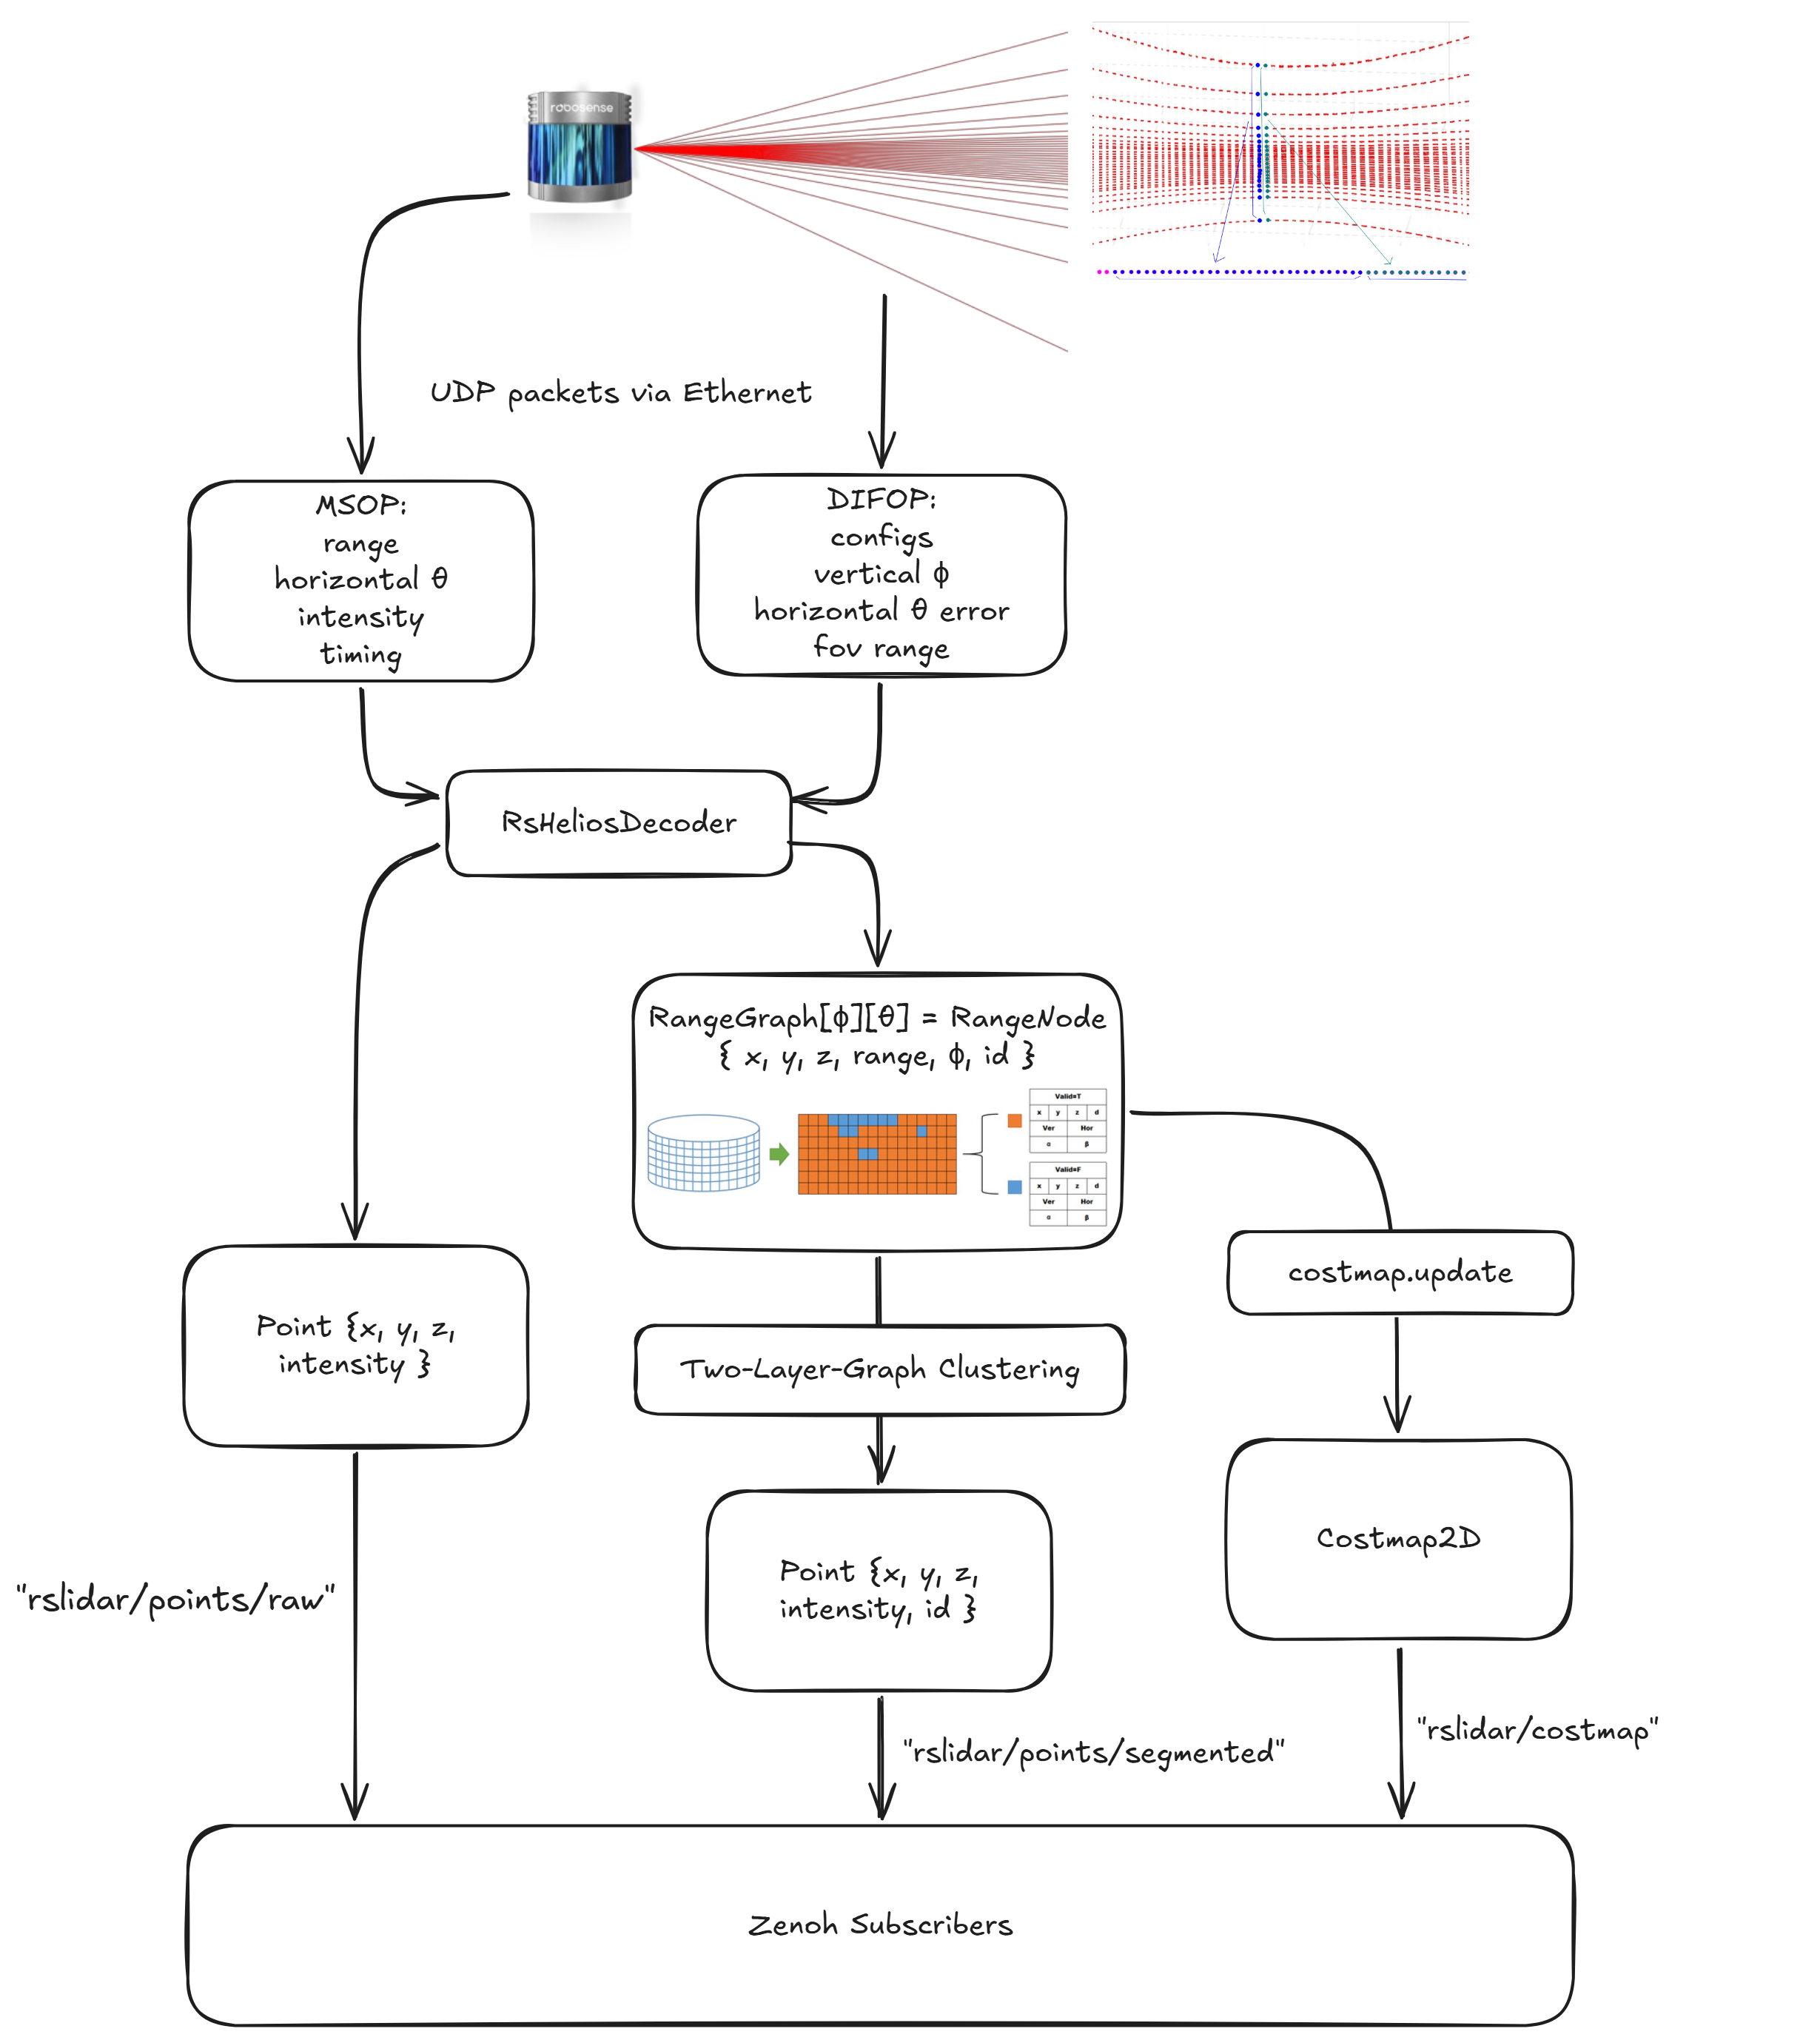
\includegraphics[width=0.95\linewidth]{low.png}
\caption{Training PL histogram with equal-frequency (left) and equal-width (right) bin edges, $K=20$.}
\label{fig:disc}
\end{figure}

\section{KLT Tracking via Intensity-Depth Fusion}
\textbf{Proposal.} The idea here is to simulate a form of camera-LiDAR sensor fusion without actually requiring synchronization between a physical camera and LiDAR.
The RoboSense Helios LiDAR outputs UDP packets containing not only vertical $\theta$ and horizontal $\phi$ firing angles of each laser, the range $r$ travelled 
prior to collision, and associated timestamps $t$, but also the reflection strength of each laser, also known as intensity. Reflection strength is dependent on the
material of the surface that each laser beam collided with. As a result, we can essentially construct a sparse inage of the environment around the sensor platform
via an intensity map. This intensity map can be passed in with associated depth information to the KLT algorithm to perform some pseudo-optical flow on a sequence 
of LiDAR scans.

\end{document}
